\documentclass[12pt]{article}

\usepackage[margin = .8in]{geometry}
\usepackage{amsmath}
\usepackage{graphicx}
\usepackage{multicol, enumerate, tabularx}

\usepackage{adjustbox}

\usepackage{fancyhdr}
\pagestyle{fancy}

\lhead{Math F113X: Numbers and Society}
\rhead{Date: \hspace{1in}}

\usepackage{tikz}
\usetikzlibrary{calc,trees,positioning,arrows,fit,shapes,through, backgrounds}
\usetikzlibrary{patterns}

\usetikzlibrary{decorations.markings}
\usetikzlibrary{arrows}

\usepackage{pgfplots}

\usepackage{longtable}
\usepackage{tabularx}

\newcommand{\ds}{\displaystyle}
\newcommand{\ans}[1][1in]{\rule{#1}{.5pt}}

\newcommand{\points}[1]{(#1 points.)}		% Trying to be lazy.

\usepackage{array}
\newcolumntype{L}[1]{>{\raggedright\let\newline\\\arraybackslash\hspace{0pt}}m{#1}}
\newcolumntype{C}[1]{>{\centering\let\newline\\\arraybackslash\hspace{0pt}}m{#1}}
\newcolumntype{R}[1]{>{\raggedleft\let\newline\\\arraybackslash\hspace{0pt}}m{#1}}
\newcommand{\red}[1]{\textcolor{red}{#1}}

\newcommand{\be}{\begin{enumerate}}
\newcommand{\ee}{\end{enumerate}}

%\topmargin -1in
%\textheight 9.5in
%\oddsidemargin -0.3in
%\evensidemargin \oddsidemargin
%\pagestyle{empty}
%%\marginparwidth 0.5in
%\textwidth 7in
%\parindent 0in

%--------------------------------------------------------------------------------------------------------------------------------------------------------------------------
%						Document
%--------------------------------------------------------------------------------------------------------------------------------------------------------------------------


\begin{document}
%\pagestyle{fancy}
\begin{center}
{\Large  Worksheet 11 (Graph Theory 3): Minimum Cost Spanning Tree}
\end{center}



\noindent \textbf{Group Names:} \hrulefill \\
%-------------------------------------------------------------------------------------------------------------
%						Assignment
%-----------------------------------------------------------------------------------------------------
\begin{enumerate}

\item Find two different spanning trees in the graph below. Draw one on each copy of the graph.

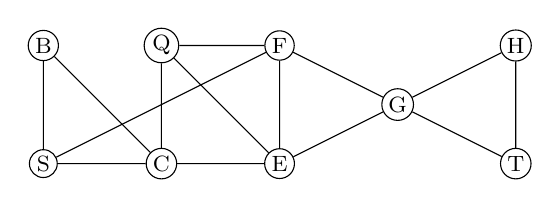
\begin{tikzpicture}[baseline=(current bounding box.center), scale=.5]
\tikzstyle{every node}=[circle, draw, fill=black!0,
                        inner sep=1pt, minimum width=10pt, font = \footnotesize]
\path (0,0) node[] (A) {S} ;
\node (B)  at (0,3) {B};
\node (C) at (3,0) {C} ;
\node (E) at (6,0) {E} ;
\node (F) at (6,3)  {F} ;
\node (D) at (3,3)  {Q};
\node (G) at (9, 1.5) {G};
\node (H) at (12, 3) {H};
\node (I) at (12, 0) {T};
\draw (A) -- (B) -- (C) -- (D) -- (F);
\draw  (F)--(G) -- (E) -- (F);
\draw (D)-- (E) --(C) --(A)--(F);
\draw (H)--(I)--(G)--(H);
\end{tikzpicture}
\hfill
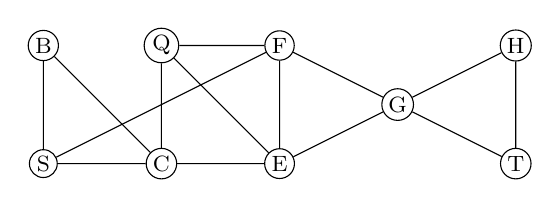
\begin{tikzpicture}[baseline=(current bounding box.center), scale=.5]
\tikzstyle{every node}=[circle, draw, fill=black!0,
                        inner sep=1pt, minimum width=10pt, font = \footnotesize]
\path (0,0) node[] (A) {S} ;
\node (B)  at (0,3) {B};
\node (C) at (3,0) {C} ;
\node (E) at (6,0) {E} ;
\node (F) at (6,3)  {F} ;
\node (D) at (3,3)  {Q};
\node (G) at (9, 1.5) {G};
\node (H) at (12, 3) {H};
\node (I) at (12, 0) {T};
\draw (A) -- (B) -- (C) -- (D) -- (F);
\draw  (F)--(G) -- (E) -- (F);
\draw (D)-- (E) --(C) --(A)--(F);
\draw (H)--(I)--(G)--(H);
\end{tikzpicture}

\item Here are four different subgraphs in a weighted graph. Graphs 1 and 2 are spanning trees.

\begin{tabularx}{\linewidth}{ X X X X}
Graph 1 & Graph 2 & Graph 3 & Graph 4 \\
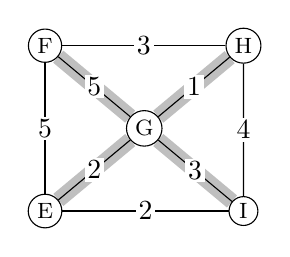
\begin{tikzpicture}[baseline=(current bounding box.center), scale=.7, xscale = .6]
\tikzstyle{vtx}=[circle, draw, fill=black!0,
                        inner sep=1.5pt, minimum width=10pt, font = \footnotesize]
 \tikzstyle{lbl}=[midway, inner sep = 1 pt, fill = white]
%\path (0,0) node[] (A) {S} ;
%\node (B)  at (0,3) {B};
\node[vtx] (E) at (6,0) {E} ;
\node[vtx] (F) at (6,3)  {F} ;
\node[vtx] (G) at (9, 1.5) {G};
\node[vtx] (H) at (12, 3) {H};
\node[vtx] (I) at (12, 0) {I};
\foreach \i/\j/\k in {F/G/5,G/E/2,E/F/5,H/I/4,I/G/3,G/H/1,F/H/3, E/I/2}{\draw (\i) -- node[lbl]{\k} (\j);}
\begin{scope}[on background layer]
\foreach \i/\j/\k in {F/G/5,G/E/2,I/G/3,G/H/1}{\draw[ gray!50, line width = 2mm] (\i) -- (\j);}
\end{scope}
\end{tikzpicture}
%%%%%%
&
%%%%%%%%
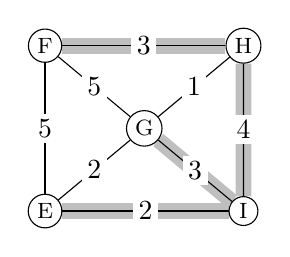
\begin{tikzpicture}[baseline=(current bounding box.center), scale=.7, xscale = .6]
\tikzstyle{vtx}=[circle, draw, fill=black!0,
                        inner sep=1.5pt, minimum width=10pt, font = \footnotesize]
 \tikzstyle{lbl}=[midway, inner sep = 2 pt, fill = white]
%\path (0,0) node[] (A) {S} ;
%\node (B)  at (0,3) {B};
\node[vtx] (E) at (6,0) {E} ;
\node[vtx] (F) at (6,3)  {F} ;
\node[vtx] (G) at (9, 1.5) {G};
\node[vtx] (H) at (12, 3) {H};
\node[vtx] (I) at (12, 0) {I};
\foreach \i/\j/\k in {F/G/5,G/E/2,E/F/5,H/I/4,I/G/3,G/H/1,F/H/3, E/I/2}{\draw (\i) -- node[lbl]{\k} (\j);}
\begin{scope}[on background layer]
\foreach \i/\j/\k in {H/I/4,F/H/3, E/I/2,I/G/3}{\draw[ gray!50, line width = 2mm] (\i) -- (\j);}
\end{scope}
\end{tikzpicture}
%%%%%%
&
%%%%%%%%
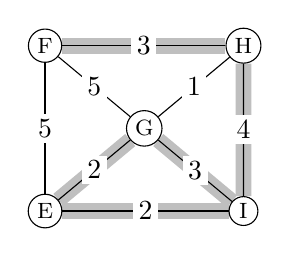
\begin{tikzpicture}[baseline=(current bounding box.center),scale=.7, xscale = .6]
\tikzstyle{vtx}=[circle, draw, fill=black!0,
                        inner sep=1.5pt, minimum width=10pt, font = \footnotesize]
 \tikzstyle{lbl}=[midway, inner sep = 2 pt, fill = white]
%\path (0,0) node[] (A) {S} ;
%\node (B)  at (0,3) {B};
\node[vtx] (E) at (6,0) {E} ;
\node[vtx] (F) at (6,3)  {F} ;
\node[vtx] (G) at (9, 1.5) {G};
\node[vtx] (H) at (12, 3) {H};
\node[vtx] (I) at (12, 0) {I};
\foreach \i/\j/\k in {F/G/5,G/E/2,E/F/5,H/I/4,I/G/3,G/H/1,F/H/3, E/I/2}{\draw (\i) -- node[lbl]{\k} (\j);}
\begin{scope}[on background layer]
\foreach \i/\j/\k in {H/I/4,F/H/3, E/I/2,I/G/3,G/E/2}{\draw[ gray!50, line width = 2mm] (\i) -- (\j);}
\end{scope}
\end{tikzpicture}
%%%%%%
&
%%%%%%%%
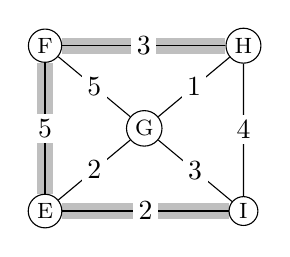
\begin{tikzpicture}[baseline=(current bounding box.center),scale=.7, xscale = .6]
\tikzstyle{vtx}=[circle, draw, fill=black!0,
                        inner sep=1.5pt, minimum width=10pt, font = \footnotesize]
 \tikzstyle{lbl}=[midway, inner sep = 2 pt, fill = white]
%\path (0,0) node[] (A) {S} ;
%\node (B)  at (0,3) {B};
\node[vtx] (E) at (6,0) {E} ;
\node[vtx] (F) at (6,3)  {F} ;
\node[vtx] (G) at (9, 1.5) {G};
\node[vtx] (H) at (12, 3) {H};
\node[vtx] (I) at (12, 0) {I};
\foreach \i/\j/\k in {F/G/5,G/E/2,E/F/5,H/I/4,I/G/3,G/H/1,F/H/3, E/I/2}{\draw (\i) -- node[lbl]{\k} (\j);}
\begin{scope}[on background layer]
\foreach \i/\j/\k in {F/H/3, E/F/5,E/I/2}{\draw[ gray!50, line width = 2mm] (\i) -- (\j);}
\end{scope}
\end{tikzpicture}
\end{tabularx}
\be
\item What is the total cost of the spanning tree in Graph 1? \ans
\item What is the total cost of the spanning tree in  Graph 2? \ans
\item Which spanning tree has smaller total cost? \ans
\item Why is the subgraph in Graph 3 not a spanning tree? \hrulefill
\vfill
\item Why is the subgraph in Graph 4 not a spanning tree? \hrulefill
\vfill
\ee

%\begin{adjustbox}{valign=t,minipage={.5\textwidth}}
%{
% \begin{tabular}{c | c}
% &
% \end{tabular}
%}
%\end{adjustbox}

%\bigskip
%\vfill

%\hfill{...continued on the back side}

\vfill

\item Use Kruskal's Algorithm to find a minimum cost spanning tree in the following graph. Break any ties by choosing the edge that comes earlier in the alphabet. (For example, edge $DC$ is the same edge as edge $CD$, and $CD$ alphabetizes earlier than $GH$.)

Construct a minimum cost spanning tree in the second graph, and keep track of the steps of the algorithm, the edges that you are using and the weights, in the table below.

\bigskip

\begin{adjustbox}{valign=t,minipage={.4\textwidth}}
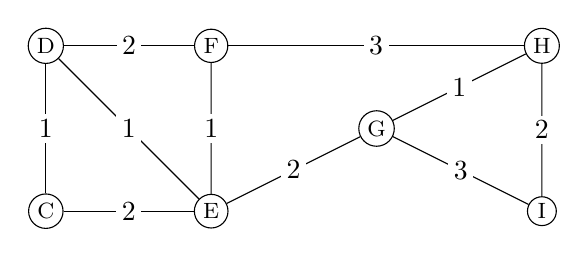
\begin{tikzpicture}[baseline=(current bounding box.center), scale=.7, ]
\tikzstyle{vtx}=[circle, draw, fill=black!0,
                        inner sep=1.5pt, minimum width=10pt, font = \footnotesize]
 \tikzstyle{lbl}=[midway, inner sep = 2 pt, fill = white]
%\path (0,0) node[] (A) {S} ;
%\node (B)  at (0,3) {B};
\node[vtx] (C) at (3,0) {C} ;
\node[vtx] (E) at (6,0) {E} ;
\node[vtx] (F) at (6,3)  {F} ;
\node[vtx] (D) at (3,3)  {D};
\node[vtx] (G) at (9, 1.5) {G};
\node[vtx] (H) at (12, 3) {H};
\node[vtx] (I) at (12, 0) {I};
%\draw (A) -- (B) -- (C) -- 
\foreach \i/\j/\k in {F/D/2,D/C/1,G/E/2,E/F/1,D/E/1,E/C/2,H/I/2,I/G/3,G/H/1,F/H/3}{\draw (\i) -- node[lbl]{\k} (\j);}
%\draw (F) -- (D) -- (C);
%\draw  (F)--(G) -- (E) -- (F);
%\draw (D)-- (E) --(C);
%\draw (H)--(I)--(G)--(H);
%\draw (F) -- (H);
\end{tikzpicture}
%\end{center}
\end{adjustbox}
%
\hfill
%
\begin{adjustbox}{valign=t,minipage={.4\textwidth}}
\begin{tikzpicture}[baseline=(current bounding box.center), scale=.7]
\tikzstyle{vtx}=[circle, draw, fill=black!0,
                        inner sep=1.5pt, minimum width=10pt, font = \footnotesize]
 \tikzstyle{lbl}=[midway, inner sep = 2 pt, fill = white]
%\path (0,0) node[] (A) {S} ;
%\node (B)  at (0,3) {B};
\node[vtx] (C) at (3,0) {C} ;
\node[vtx] (E) at (6,0) {E} ;
\node[vtx] (F) at (6,3)  {F} ;
\node[vtx] (D) at (3,3)  {D};
\node[vtx] (G) at (9, 1.5) {G};
\node[vtx] (H) at (12, 3) {H};
\node[vtx] (I) at (12, 0) {I};
%\foreach \i/\j/\k in {F/D/2,D/C/1,F/G/5,G/E/2,E/F/5,D/E/1,E/C/2,H/I/4,I/G/3,G/H/1,F/H/3, E/I/2}{\draw (\i) -- node[lbl]{\k} (\j);}
\end{tikzpicture}

%\end{center}
\end{adjustbox}
%
%\begin{adjustbox}{valign=t,minipage={.25\textwidth}}

\bigskip

\begin{adjustbox}{valign=t,minipage={.6\linewidth}}
\begin{tabular}{ c | p{1.5in} | p{1.5in}}
Used? &edges & weights\\ \hline
& \\
& \\
& \\& \\& \\& \\& \\& % \\& \\& \\
 \end{tabular}
 \end{adjustbox}
 
 What is the total cost of the spanning tree you found? \ans
 
\newpage

\item Use Kruskal's Algorithm to determine a minimum cost spanning tree in the following graph. 

Break any ties by choosing the edge that comes earlier in the alphabet. (For example, edge $DC$ is the same edge as edge $CD$, and $CD$ alphabetizes earlier than $GH$.)

Construct a minimum cost spanning tree in the second graph, and keep track of the steps of the algorithm, the edges that you are using and the weights, in the table below.

For convenience, I have listed the edges of the graph in sorted order for you.

\begin{adjustbox}{valign=t,minipage={.4\textwidth}}
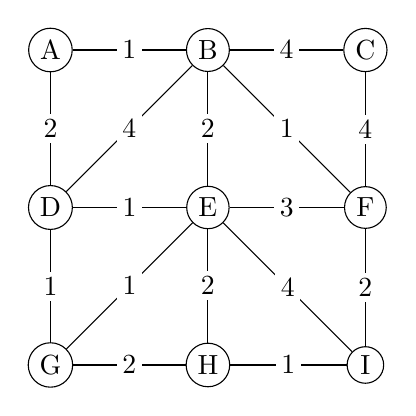
\begin{tikzpicture}
\tikzstyle{vtx}=[draw, circle, inner sep = 2 pt, node distance=2cm]
\tikzstyle{lbl}=[midway, inner sep = 2 pt, fill = white]

\node[vtx] (A)  {A};
\node[vtx, right of =  A] (B) {B};
\node[vtx, right of = B] (C) {C};
\node[vtx, below of = A] (D) {D};
\node[vtx, below of = B] (E) {E};
\node[vtx, below of = C] (F) {F};
\node[vtx, below of = D] (G) {G};
\node[vtx, below of = E] (H){H};
\node[vtx, below of = F] (I){I};
\draw (A) -- node[lbl]{1} (B) -- node[lbl]{4} (C) -- node[lbl]{4} (F) -- node[lbl]{2} (I) -- node[lbl]{1} (H) -- node[lbl]{2} (G) -- node[lbl]{1} (D)-- node[lbl]{2} (A);
\draw (B) --node[lbl] {2} (E) --node[lbl] {1} (D);
\draw (F) --node[lbl] {3} (E) --node[lbl] {2} (H);
\draw (E) --node[lbl] {1} (G);
\draw (E)--node[lbl] {4} (I);
\draw (B) -- node[lbl] {4} (D);
\draw (B) -- node[lbl] {1} (F);
\end{tikzpicture}
\end{adjustbox}
%%%
\hfill
%%%%%%%%
\begin{adjustbox}{valign=t,minipage={.4\textwidth}}
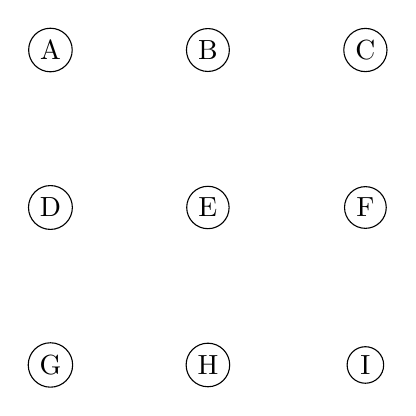
\begin{tikzpicture}
\tikzstyle{vtx}=[draw, circle, inner sep = 2 pt, node distance=2cm]
\tikzstyle{lbl}=[midway, inner sep = 2 pt, fill = white]

\node[vtx] (A)  {A};
\node[vtx, right of =  A] (B) {B};
\node[vtx, right of = B] (C) {C};
\node[vtx, below of = A] (D) {D};
\node[vtx, below of = B] (E) {E};
\node[vtx, below of = C] (F) {F};
\node[vtx, below of = D] (G) {G};
\node[vtx, below of = E] (H){H};
\node[vtx, below of = F] (I){I};
%\draw (A) -- node[lbl]{1} (B) -- node[lbl]{4} (C) -- node[lbl]{3} (F) -- node[lbl]{2} (I) -- node[lbl]{6} (H) -- node[lbl]{5} (G) -- node[lbl]{1} (D)-- node[lbl]{2} (A);
%\draw (B) --node[lbl] {1} (E) --node[lbl] {1} (D);
%\draw (F) --node[lbl] {8} (E) --node[lbl] {2} (H);
%\draw (E) --node[lbl] {1} (G);
%\draw (E)--node[lbl] {4} (I);
\end{tikzpicture}
\end{adjustbox}

\vspace{1cm}

\begin{adjustbox}{valign=t,minipage={.1\linewidth}}
\begin{tabular}{ c | c}
Sorted edges & weight\\ \hline
$AB$ & 1 \\
$BF$ & 1 \\
$DE$ & 1 \\
$DG$ & 1\\
$EG$ & 1\\
$HI$ & 1 \\
$AD$ & 2 \\
$BE$ & 2 \\ 
$EH$ & 2\\
$FI$ & 2\\
$GH$ & 2\\
$BC$ & 4 \\
$BD$ & 4 \\ 
$CF$ & 4\\
$EI$ & 4 \\

 \end{tabular}
 \end{adjustbox}
 %%%%%%
 \hfill
 %%%%%%%
\begin{adjustbox}{valign=t,minipage={.6\linewidth}}
\begin{tabular}{ c | p{1.5in} | p{1.5in}}
Used? &edges & weights\\ \hline
& \\
& \\
& \\& \\& \\& \\& \\& \\& \\& \\& \\& \\ & \\& \\
 \end{tabular}
 \end{adjustbox}

 
\vspace{1cm}

 
 What is the total cost of the spanning tree you found? \ans
 
\end{enumerate}

\end{document}

%-------------------------------------------------------------------------------------------------------------------------------------------------------------------------------------------------------------------

%%% Local Variables:
%%% mode: latex
%%% TeX-master: t
%%% End:
